\documentclass{article}

\usepackage{hyperref}
\hypersetup{
    colorlinks=true,
    linkcolor=blue,
    filecolor=magenta,      
    urlcolor=cyan,
}

% for including notebooks
\usepackage{pdfpages}
\usepackage{fancyhdr}
\usepackage{extramarks}
\usepackage{amsmath}
\usepackage{amsthm}
\usepackage{amsfonts}
\usepackage{tikz}
\usepackage{float}
\usepackage[plain]{algorithm}
\usepackage{algpseudocode}
\usepackage{caption}
\usepackage{subcaption}
\usepackage[toc,page]{appendix}
\usepackage{siunitx}
\usepackage{footnote}

\usepackage{listings}
\usepackage{color} 
\definecolor{mygreen}{RGB}{28,172,0} 
\definecolor{mylilas}{RGB}{170,55,241}

\lstset{
    basicstyle=\scriptsize\sffamily\color{black},
    frame=single,
    numbers=left,
    showspaces=false,
    showstringspaces=false,
    tabsize=1
}
\lstset{language=Matlab,%
    %basicstyle=\color{red},
    breaklines=true,%
    morekeywords={matlab2tikz},
    keywordstyle=\color{blue},%
    morekeywords=[2]{1}, keywordstyle=[2]{\color{black}},
    identifierstyle=\color{black},%
    stringstyle=\color{mylilas},
    commentstyle=\color{mygreen},%
    showstringspaces=false,%without this there will be a symbol in the places where there is a space
    numbers=left,%
    numberstyle={\tiny \color{black}},% size of the numbers
    numbersep=9pt, % this defines how far the numbers are from the text
    emph=[1]{for,end,break},emphstyle=[1]\color{red}, %some words to emphasise
    %emph=[2]{word1,word2}, emphstyle=[2]{style},    
}

\topmargin=-0.45in
\evensidemargin=0in
\oddsidemargin=0in
\textwidth=6.5in
\textheight=9.0in
\headsep=0.25in


\linespread{1.1}

\pagestyle{fancy}
\fancyhf{}
\lhead{\hmwkAuthorName}
\chead{\hmwkClass: \hmwkTitle}
\rhead{\leftmark}
\lfoot{\lastxmark}
\cfoot{\thepage}

\renewcommand\headrulewidth{0.4pt}
\renewcommand\footrulewidth{0.4pt}

\setlength\parindent{0pt}

\newcommand{\hmwkTitle}{Assignment \ 1}
\newcommand{\hmwkDueDate}{March 10, 2020}
\newcommand{\hmwkClass}{Introduction to AI}
\newcommand{\hmwkClassInstructor}{Dr. Joseph Brown}
\newcommand{\hmwkAuthorName}{\textbf{Artem Bakhanov (B18-03)}}

%
% Title Page
%

\title{
    \vspace{2in}
    \textmd{\textbf{\hmwkClass:\ \hmwkTitle}}\\
    \normalsize\vspace{0.1in}\small{Due\ on\ \hmwkDueDate\ at 11:59pm}\\
    \vspace{0.1in}\large{\textit{\hmwkClassInstructor\ }}
    \vspace{3in}
}

\author{\hmwkAuthorName}
\date{}

\begin{document}

\maketitle

\pagebreak

\tableofcontents

\pagebreak

\section{Introduction}
\subsection{General information}
    The assignment is solved by me, Artem Bakhanov, a student of Innopolis University. If you have any question regarding any part of this document and other provided materials, you can contact me via email: \href{mailto:a.bahanov@innopolis.university}{a.bahanov@innopolis.university}.\\
    In this assignment, I used SWI Prolog of version 8.0.3-1. It can be easily downloaded from the official \href{https://www.swi-prolog.org/download/stable}{website}. I highly recommend you to use \href{https://marketplace.visualstudio.com/items?itemName=arthurwang.vsc-prolog}{VCS-Prolog} extension for Visual Studio Code. \\
\texttt{main.pl} - Prolog file with program\\
\texttt{/tests} - Directory with input tests\\

\subsection{Running the code}
To run the program, you need to execute \url{main.pl} file and run the following query: \texttt{?- start(Alg, Test, [ShowMap]).} where \texttt{Alg} is 0, 1, or 2, which stands for Backtracking Search, Random Search, and Improved BFS (IBFS), respectively; \texttt{Test} is the number of input test to be executed; \texttt{ShowMap} - if \texttt{true} the map and the solution path will be printed out the standard output. The result will be printed to the standard output of the interpreter. Note that I used the same output conventions as it is stated in the assignment text. \textbf{Important!} The directory \texttt{/tests} should exist for running the program.
\begin{figure}[ht]
   	 \centering
     \begin{subfigure}[b]{0.45\textwidth}
         \centering
         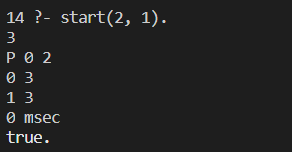
\includegraphics[width=\textwidth]{images/image4.png}
         \caption{Running IBSF on test 1 without map}
         \label{fig:output1}
     \end{subfigure}
     \hfill
     \begin{subfigure}[b]{0.45\textwidth}
         \centering
         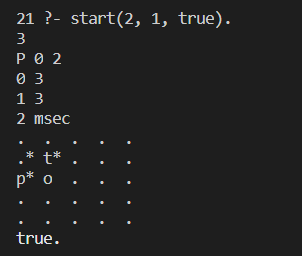
\includegraphics[width=\textwidth]{images/image5.png}
         \caption{Running IBSF on test 1 with map}
         \label{fig:output2}
     \end{subfigure}
     \caption{Examples of output.}
\end{figure} 

\subsection{Tests}
All the tests are created by me (except for the first one, which was taken from the assignment text). You can find them in the directory called "tests". They are simple prolog files with predefined predicates. Note that I use predicates \texttt{player(+Position)}, \texttt{orc(+Position)}, and \texttt{touchdown(+Position)} for defining players', orcs' and touchdowns positions respectively, where \texttt{Position} is a position predicate \texttt{p(X, Y)} with X and Y coordinates. X-axis is a horizontal axis directed to the right, Y-axis is a vertical one directed upward (please see figures ~\ref{fig:test1} and ~\ref{fig:test2}). You can find all the tests in the appendix ~\ref{appendix:tests}. All the tests are created in such a way that they touch edge cases.
\lstinputlisting[caption=Test 1={lst:listing1}, language=Prolog]{tests/input1.pro}

\begin{figure}[ht]
   	 \centering
     \begin{subfigure}[b]{0.45\textwidth}
         \centering
         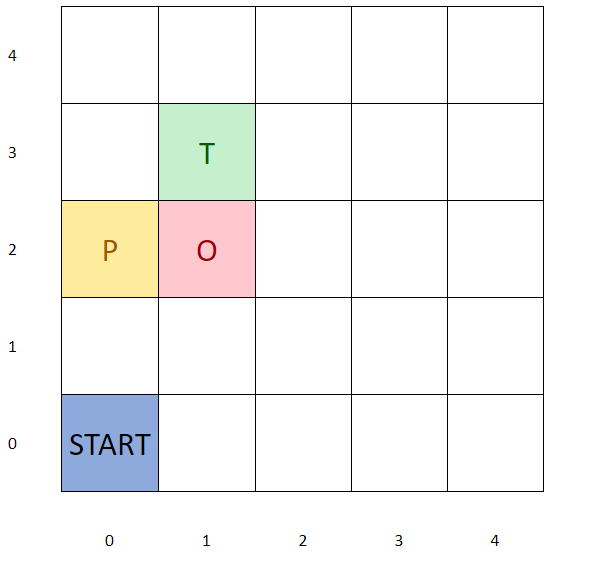
\includegraphics[width=\textwidth]{images/image1.png}
         \caption{Test 1}
         \label{fig:test1}
     \end{subfigure}
     \hfill
     \begin{subfigure}[b]{0.45\textwidth}
         \centering
         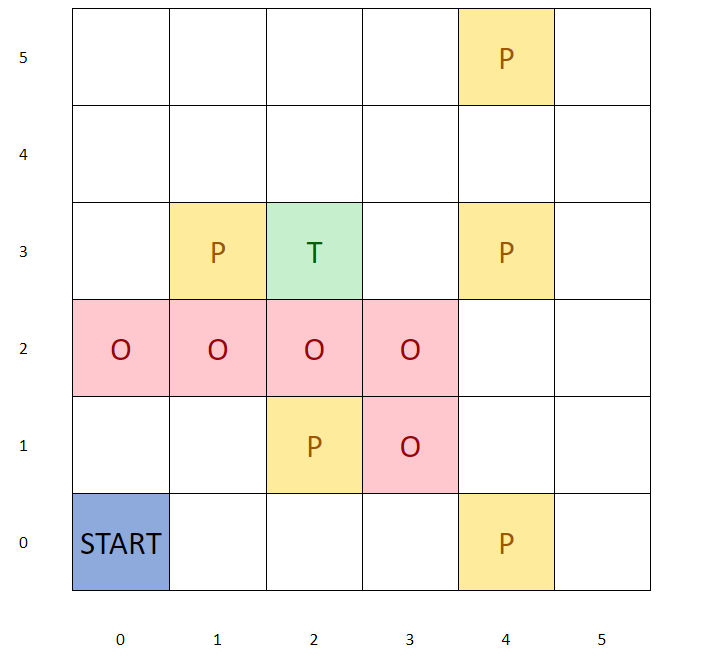
\includegraphics[width=\textwidth]{images/image2.png}
         \caption{Test 2}
         \label{fig:test2}
     \end{subfigure}
     \caption{Examples of tests.}
\end{figure}
Here and throughout I mark players (humans) as P (yellow), orcs as O (red), touchdowns as T (green). The start is always situated at $(0, 0)$. By the conventions, player at the start cell is not explicitly specified in the input files.

\section{Algorithms}
\subsection{Backtracking Algorithm}
I implemented the backtracking algorithm using the Prolog Tree. The algorithm finds the first solution and returns it. There is no randomness in the implementation, so the algorithm tries to traverse the map spirally. In the backtracking search, the algorithm tries all the possible movements, including ball passes (if it was not performed earlier).\\
There are several assumptions I made during coding the algorithm.
\begin{enumerate}
	\item There is no need to return to a cell where the ball was before (i.e. duplicated move).
	\item Since the ball cannot return to any previous position, there is no need to move players. All the positions are static predicates.
	\item There is no need to pass a ball over a cell where it was before. For example, if player 1 passes a ball from $(2, 1)$ to player 1 located in $(2, 5)$ after player 1 came to $(2, 1)$ from $(2, 3)$, then there is no reason no make such a pass because it could be made earlier.
	\item Handoff is a move but with 0 cost.
	\item The start position of the ball is not saved while performing the backtracking search since the ball cannot enter $(0, 0)$ twice and exit from there because of forbidden duplicated moves.
\end{enumerate}
A very important metric of the algorithm is its time complexity. Since the algorithm is exponentially complex its execution time can be high on the big maps (e.g. 10*10). On big maps with "unusual" field configuration, the algorithm needs a lot of time. For instance, the algorithm does not work on test 7 faster than 5 minutes (I did not run the algorithm for a longer time). Note that the problem with the test is just a \texttt{move} predicate order. The algorithm goes in this order: it tries to pass the ball from upward clockwise, then it tries to move a player from upward clockwise.

\subsection{Random Search}
The random search is very similar to the backtracking search except for the implementation of \texttt{move} predicate. I create new predicate \texttt{select\_random\_move(...)}, which literally selects only one move at a time (I used cut to avoid backtracking behaviour). The second difference is that the random search performs exactly 100 moves in one round. I simulate 100000 rounds and select the best solution. I used the same assumptions as I used for backtracking search.\\
The time complexity of the algorithm is always constant since the algorithm performs the same amount of work for any input (100 moves for each round). 

\subsection{Improved BFS (IBFS)}
The third algorithm I implemented was actually an experiment that turned out to be very effective and fast. The algorithm is really similar to BFS but I added new features to improve its time and space performance. The idea of the algorithm is that it does not go in depth. Each iteration (recursive call) it searches new possibilities to move for a "history" from the queue (a simple Prolog list). 
\\By "history" I mean some game state that is not finished yet; it contains current ball position, the number of moves taken, the cost of the path (i.e. depth), information about ball passes, and the path itself. The initial "history" is \texttt{history(0, p(0, 0), true, 0, 0, [])}, which means that the "history" has id 0, current ball position is $(0, 0)$, ball pass has not been performed yet, cost and number of steps are 0, and the path is empty. New possibilities to move are actually histories that can be created after exactly one move. 
\\Let us give you an example for test 1 (see figure \ref{fig:test1}). The algorithm searches all the possibilities to move from the initial state. All the possible moves here are: go to $(0, 1)$ and $(1, 0)$ and pass the ball to player at $(0, 2)$; therefore new "histories" will be:
\begin{lstlisting}[caption=Histories of depth 1={lst:listing2}, language=Prolog]
	history(1,p(0,2),false,1,1,[pass,p(0,2)]);
	history(2,p(0,1),true,1,1,[move,p(0,1)]);
	history(3,p(1,0),true,1,1,[move,p(1,0)]).
\end{lstlisting}
These histories are pushed into a queue and passed to the next recursive call. In the next recursive iteration the algorithm pops the a history and tries to find its child histories and pushes them to the queue. For example in the second iteration there will be the following histories:
\begin{lstlisting}[caption=History of depth 2={lst:listing2}, language=Prolog]
	history(4,p(0,3),false,2,2,[move,p(0,3),pass,p(0,2)]).
\end{lstlisting}

The algorithm might seem very similar to the backtracking search but there are some additional assumptions that were made for this algorithm working significantly faster:
\begin{enumerate}
	\item If a history's cost is more or equal to another history's cost provided they have the same ball position (or the second one had less cost when went through the cell), then the first history can be discarded except for the situation, described in the second assumption.
	\item If there are two histories reaches a cell, but a ball pass was performed only in the first one and their costs are the same, then BOTH histories MUST be considered.
	\item The cost of the ball pass is a Manhattan distance between two players minus 1 ($d_1(p_1, p_2) - 1$). (Note: ball pass is considered as one move when it comes to calculating the number of moves). The cost of handoff is 0.
\end{enumerate}
The first assumption is quite simple. If a history reaches a cell that was reached faster (with smaller cost), there is no need to find the next histories, since another history already has a better path.\\
The second assumption is an edge case of the first one. If it is possible to come to a cell with the same cost as another history had in this cell, but with a ball pass, then it is expedient to continue searching. It might help in situations when a ball pass is made too early, but it is needed later to pass diagonal orcs wall. If such a history is discarded, then the solution will not be found.\\
The third assumption is about moves costs. While the cost of the regular move (up, down, right, left without handoff) is 1, the cost of a ball pass is a Manhattan distance minus one, since there are AT MOST such an amount of steps needed to be performed to reach the cell where the ball was passed to. Subtracting one is used since the last move's cost is 0 (handoff).\\
The time complexity of the algorithm is very small due to its properties. It does not go in depth but trying to find the next moves for one-depth "histories". Full statistical analysis is presented below.
\section{Algorithms Analysis}
Let us compare all the algorithms that were presented above. I used the following metrics: execution time (ET; measured in milliseconds), the number of nodes in the prolog tree (NN), and optimality of produced solutions (PC).\\
It is important to mention that all the inputs were tested on my computer (Dell Inspiron 7577,  Intel Core i7-7700HQ 33, 16Gb DDR4 SDRAM with 2400 MHz memory speed). On other computers, execution time can be different.\\
Note that in case of backtracking search the number of nodes is a number of any intermediate recursive calls including unsuccessful ones; the number of runs of random search multiplied by the number of moves since only one move is selected at a time and there is no branching in the algorithm; the number of histories considered by improved BSF search. 

\begin{savenotes}
\begin{table}[H]
\centering
\begin{tabular}{|l|l|l|l|l|l|l|l|l|l|l|}
\hline
 &
  \multicolumn{3}{l|}{\textbf{Backtracking}} &
  \multicolumn{3}{l|}{\textbf{Random}} &
  \multicolumn{3}{l|}{\textbf{Improved BFS}} &
   \\ \hline
\begin{tabular}[c]{@{}l@{}}Metrics/\\ Test\#\end{tabular} &
  ET \footnote{Measured in msec.} &
  NN &
  PC &
  ET &
  NN &
  PC &
  ET &
  NN &
  PC &
  \textbf{Optimal path} \\ \hline
1  & 0.5   & 17                      & 17 & 35  & $\leq 10^7$ & 3.5 & 2   & 32  & 3  & 3  \\ \hline
2  & 0.7   & 30                      & 8  & 39  & $\leq 10^7$ & 9.6 & 2   & 58  & 5  & 5  \\ \hline
3  & 0.3   & 20                      & 20 & -   & $\leq 10^7$ & -   & 0.5 & 21  & 20 & 20 \\ \hline
4  & -     & \textgreater 16 200 000\footnote{Were run for 2 minutes. $\SI{120000}{\milli\second} \times 135 nodes/msec$} & -  & -   & $\leq 10^7$ & -   & 23  & 116 & 10 & 10 \\ \hline
5  & -     & \textgreater 16 200 000 & -  & 71  & $\leq 10^7$ & 6.8 & 8   & 192 & 5  & 5  \\ \hline
6  & -     & \textgreater 16 200 000 & -  & -   & $\leq 10^7$ & -   & 8   & 304 & 9  & 9  \\ \hline
7  & 37000 & 4838138                 & 9  & -   & $\leq 10^7$ & -   & 4   & 89  & 5  & 5  \\ \hline
8  & 1     & 43                      & 16 & 471 & $\leq 10^7$ & 8   & 2   & 35  & 8  & 8  \\ \hline
9  & 0.6   & 54                      & 27 & 179 & $\leq 10^7$ & 13  & 0.8 & 73  & 8  & 8  \\ \hline
10 & 15    & 2242                    & 12 & -   & $\leq 10^7$ & -   & 2.5 & 60  & 11 & 11 \\ \hline
11 & 6     & 617                     & 10 & 35  & $\leq 10^7$ & 1   & 10  & 135 & 1  & 1  \\ \hline
12 & 4     & 388                     & 49 & 514 & $\leq 10^7$ & 22  & 35  & 285 & 10 & 10 \\ \hline
13 & 34    & 1601                    & -  & 575 & $\leq 10^7$ & -   & 1   & 16  & -  & -  \\ \hline
14 & 1     & 108                     & -  & 575 & $\leq 10^7$ & -   & 1   & 7   & -  & -  \\ \hline
\end{tabular}
\caption{Metrics comparison.}
\label{tab:metrics}
\end{table}
\end{savenotes}

As you can see in the table \ref{tab:metrics}, IBFS show the best performance for all the metrics. It always finds the best solution with a very small amount of tree nodes. For example in tests 4, 5, 6, 7 the number of nodes in backtracking algorithm is very high and hence its execution time is big (note that the algorithm did not give any solution for tests 4, 5, 6 within 2 minutes). In these tests, IBFS performed well.\\
Since backtracking and random searches do not work well on big tests, I analyzed their performance on tests that are small enough. I did not consider random search in the t-test since it does not give persistent solutions. The p-value for different metrics are presented below:
\begin{align}
	p_{ET} &= 0.170403624 \\
	p_{NN} &= 0.170216341 \\
	p_{OP} &= 0.001435355
\end{align}
Note that $p_{OP}$ is a p-value of optimality. The optimaly is calculated as follows: $O(X_i) = \frac{OPT(X_i)}{PC_{alg}(X_i)}$, where $OPT(X_i)$ is the optimal path cost and $PC_{alg}(x_i)$ is the path cost found with algorithm $alg$. \\
As one can see, the number of nodes and execution time do not differ significantly, unlike the optimality. 
\subsection{Conclusion}
From this analysis we can conclude that generally these algorithms do not differ much on small maps. For bigger maps Improved BFS is unambiguously better.

\section{Advanced Team with Extended Visibility}
\subsection{Backtracking Algorithm}
There is no improvement of the algorithm since it works like trial and error methods. It \textbf{tries}, if no success, it rolls back and tries another way. 
\subsection{Random Search}
Random search will not get any improvement too, since it takes purely random moves, which does not depend on the environment.
\subsection{Improved Backtracking Search}
The situation is the same for this search as for the backtracking search. Since I do not use any heuristic function, extended visibility does not help at all.
\subsection{Conclusion}
There is no difference when it comes to the distance of visible objects; therefore there is no improvement in the algorithms' time complexity. These methods will not make unsolvable map solvable and vice versa.
It is important to mention that for some algorithms, extended visibility might help to improve its performance. The very obvious examples of such algorithms are A* (heuristic function) and Tabu (Tabu lists can be created without visiting certain cells) searches.

\section{Hard and Impossible Maps}
\label{section:impossible-maps}
There are different hard or impossible maps for different algorithms. 
By almost impossible map I mean the map that has a solution but it is hard to find wit a particular algorithm. Impossible map is a map without solution.
\subsection{Backtracking Algorithm}
In the case of this algorithm, it is hard to find a solution when the map forces player to start freely move from the center of the map. Example of such a map is test 4 that is shown on the picture below. As you can see, we can treat the start of the field at $(4, 0)$ where the algorithm literally starts from. Since the order of movements is from up to the left (clockwise), the algorithm will be stuck in the $X = [5, 10]$ area before it goes to the left. The algorithm did not finish in 2 minutes (more than $15 \times 10^6$ nodes in the Prolog tree).

\begin{figure}[ht]
   	 \centering
     \begin{subfigure}[b]{0.45\textwidth}
         \centering
         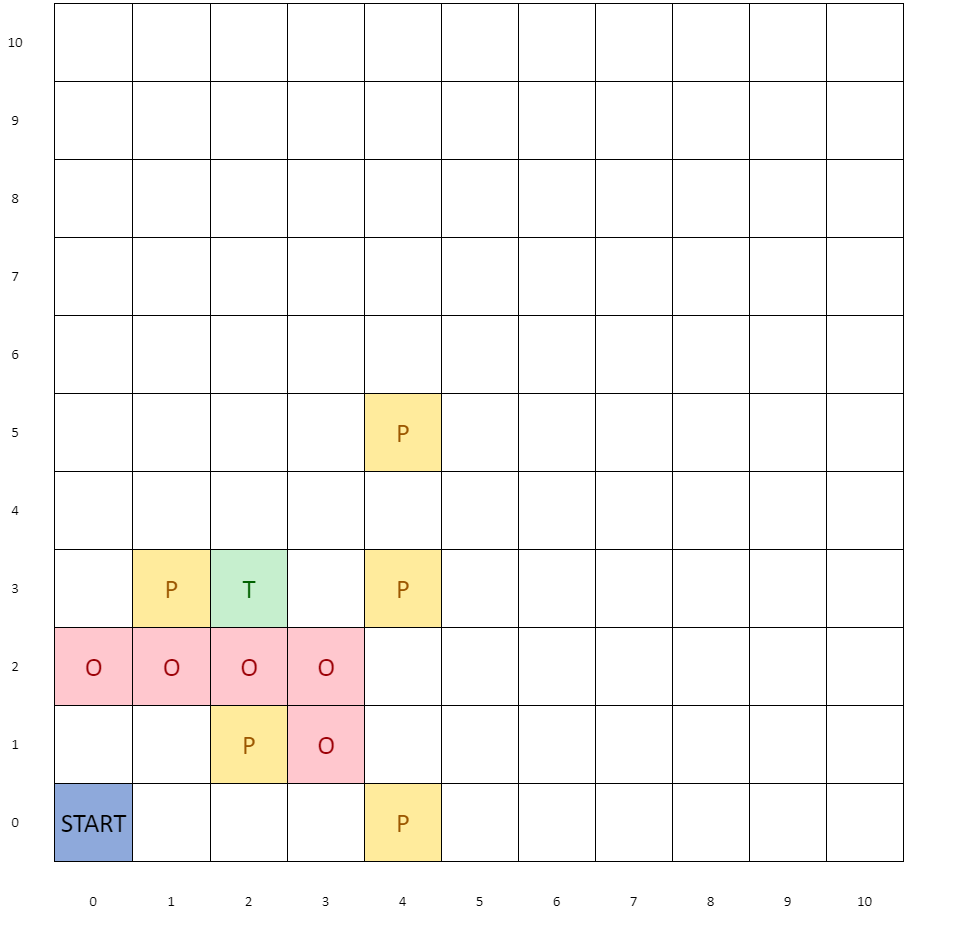
\includegraphics[width=\textwidth]{images/image3.png}
         \caption{Test 4}
         \label{fig:test4}
     \end{subfigure}
     \hfill
     \begin{subfigure}[b]{0.45\textwidth}
         \centering
         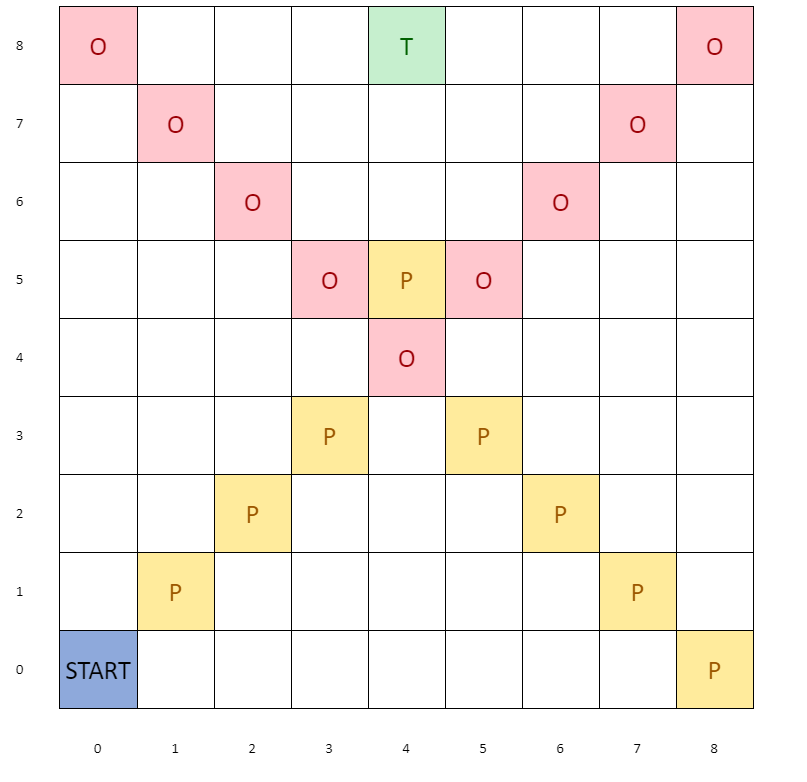
\includegraphics[width=\textwidth]{images/test5.png}
         \caption{Test 5}
         \label{fig:test5}
     \end{subfigure}
     \caption{Examples of almost impossible maps (Backtracking)}
\end{figure}
The common property of such maps is that there is a critical point in the middle of the map. By critical point I mean any cell on the map where the game literally starts (like in test 4) or there is a point in the middle of the map where a ball pass should be performed. 
\subsection{Random Search}
\begin{figure}[H]
   	 \centering
     \begin{subfigure}[b]{0.40\textwidth}
         \centering
         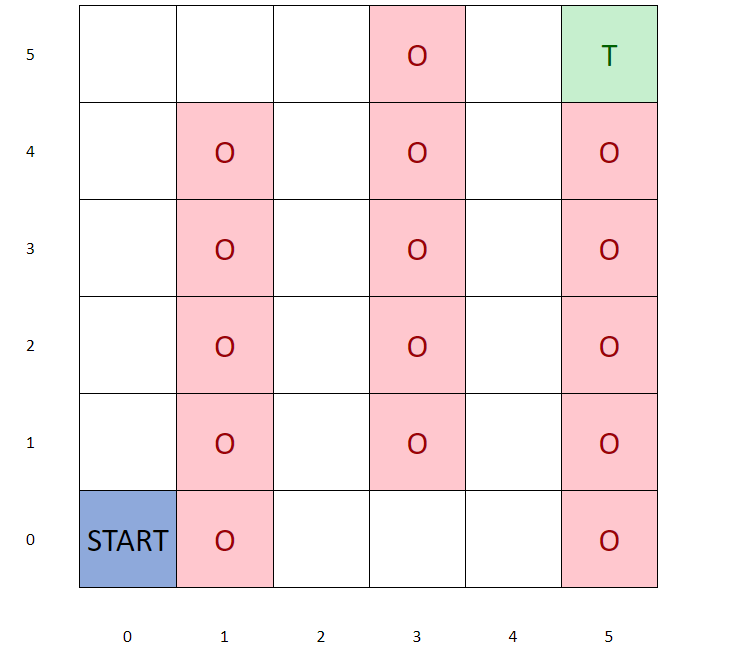
\includegraphics[width=\textwidth]{images/test3.png}
         \caption{Test 3}
         \label{fig:test3}
     \end{subfigure}
     \hfill
     \begin{subfigure}[b]{0.40\textwidth}
         \centering
         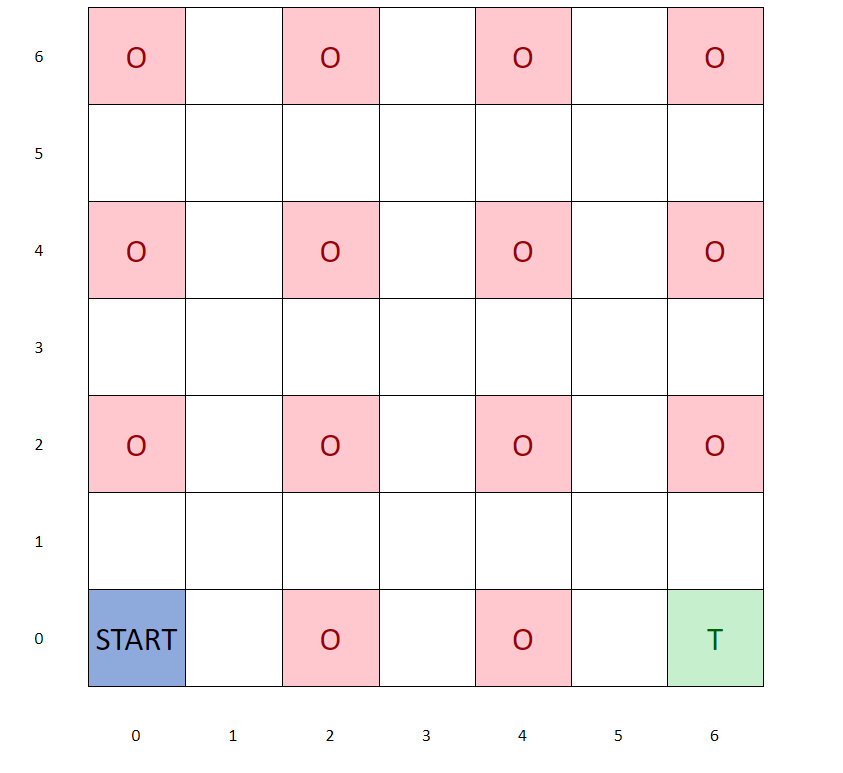
\includegraphics[width=\textwidth]{images/test8.png}
         \caption{Test 8}
         \label{fig:test8}
     \end{subfigure}
     \caption{Examples of almost impossible maps (Random search)}
\end{figure}
Random search algorithm does not work on maps with big number of orcs since there is higher probability to make a unsuccessful move. For instance, on tests 3 and 8 random search was restarted several times and yielded no result. Note that such algorithms are very easy for backtracking algorithm. Another type of almost impossible maps are just big enough maps (8*8 or more). 
\subsection{Improved BFS}
There is no "almost impossible" map for the Improved BFS algorithm since all the 20*20 maps are easy for BFS.
\subsection{Impossible maps}
Impossible maps are the same for all the algorithms. There is several types of impossible maps. Among them:
\begin{enumerate}
	\item Map without any touchdown point.
	\item Map with an orc at the starting position or at position of touchdown(s).
	\item Map with a wall of orcs around touchdown point that cannot be handled with a ball pass.
	\item Map where two or more ball passes must be performed.
\end{enumerate}
\begin{figure}[H]
   	 \centering
     \begin{subfigure}[b]{0.40\textwidth}
         \centering
         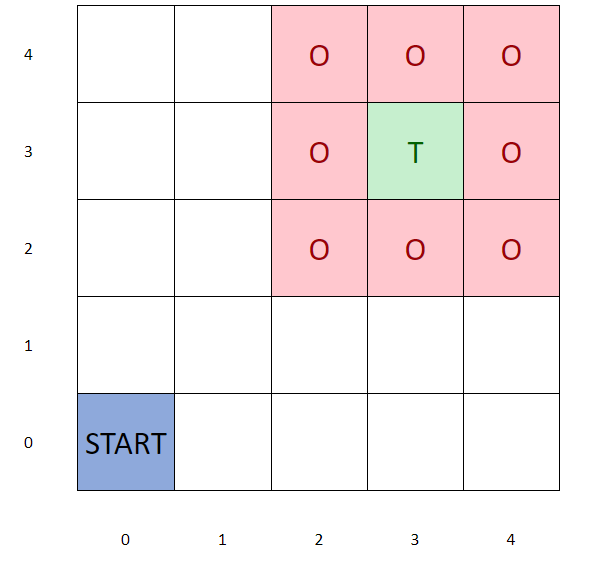
\includegraphics[width=\textwidth]{images/test13.png}
         \caption{Test 13}
         \label{fig:test13}
     \end{subfigure}
     \hfill
     \begin{subfigure}[b]{0.41\textwidth}
         \centering
         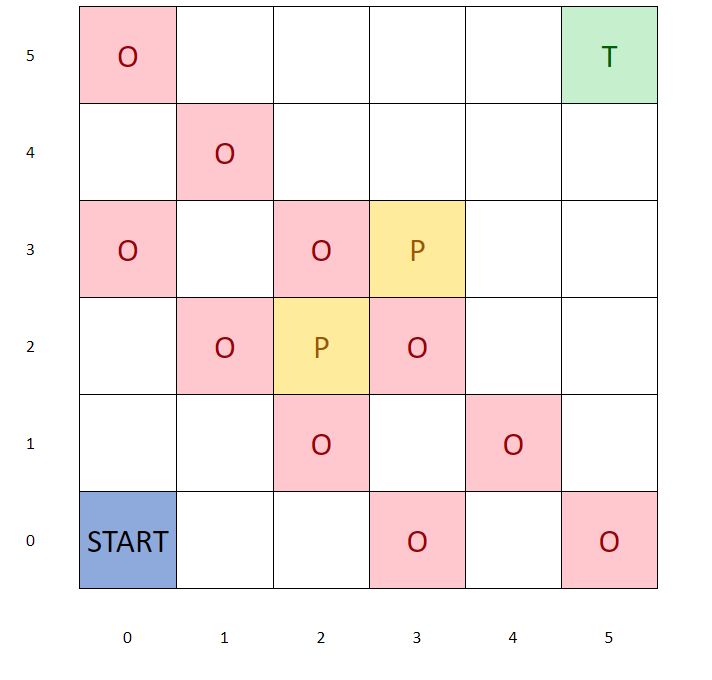
\includegraphics[width=\textwidth]{images/test14.png}
         \caption{Test 14}
         \label{fig:test14}
     \end{subfigure}
     \caption{Examples of impossible maps (All algorithms)}
\end{figure}
\begin{appendices}
\section{Input Tests}
\label{appendix:tests}
Below you can find all the tests images. Tests 9 - 12 are randomly generated. Tests 4, 5, and 6 are created for testing backtracking algorithm and its properties. Test 3 and 8 are made for testing random search. Tests 13 and 14 are impossible maps.
\begin{figure}[H]
   	 \centering
     \begin{subfigure}[b]{0.45\textwidth}
         \centering
         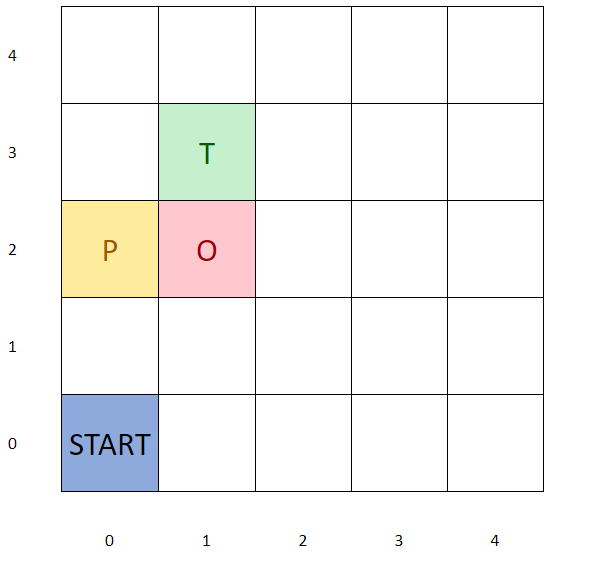
\includegraphics[width=\textwidth]{images/image1.png}
         \caption{Test 1}
         \label{fig:test13}
     \end{subfigure}
     \hfill
     \begin{subfigure}[b]{0.45\textwidth}
         \centering
         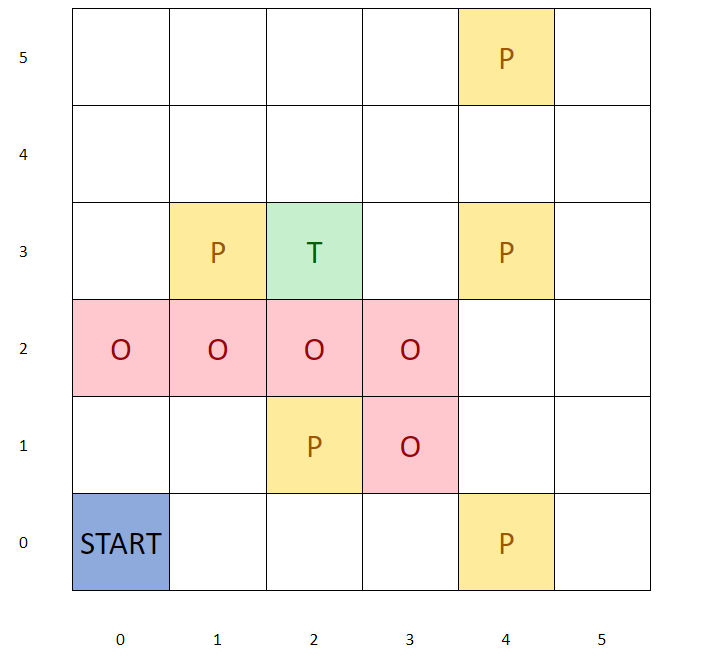
\includegraphics[width=\textwidth]{images/image2.png}
         \caption{Test 2}
         \label{fig:test14}
     \end{subfigure}
\end{figure}

\begin{figure}[H]
   	 \centering
     \begin{subfigure}[b]{0.45\textwidth}
         \centering
         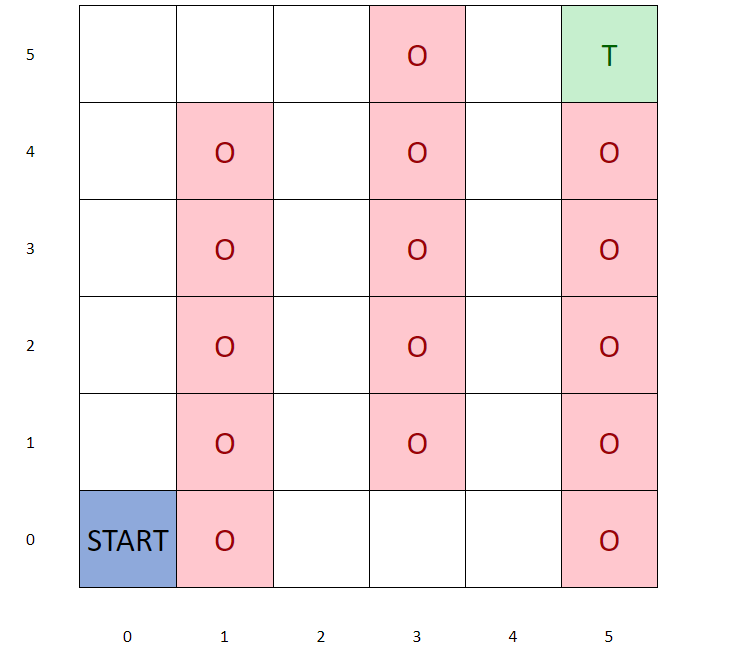
\includegraphics[width=\textwidth]{images/test3.png}
         \caption{Test 3}
         \label{fig:test13}
     \end{subfigure}
     \hfill
     \begin{subfigure}[b]{0.45\textwidth}
         \centering
         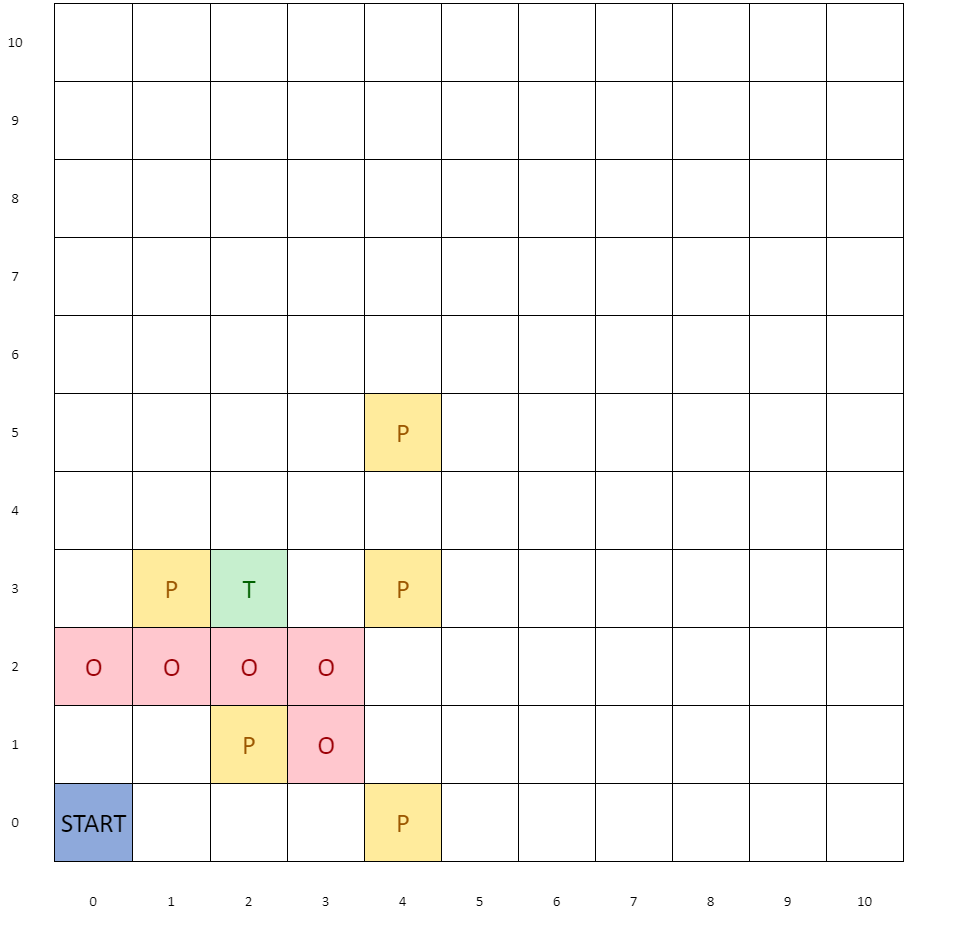
\includegraphics[width=\textwidth]{images/image3.png}
         \caption{Test 4}
         \label{fig:test14}
     \end{subfigure}
\end{figure}

\begin{figure}[H]
   	 \centering
     \begin{subfigure}[b]{0.45\textwidth}
         \centering
         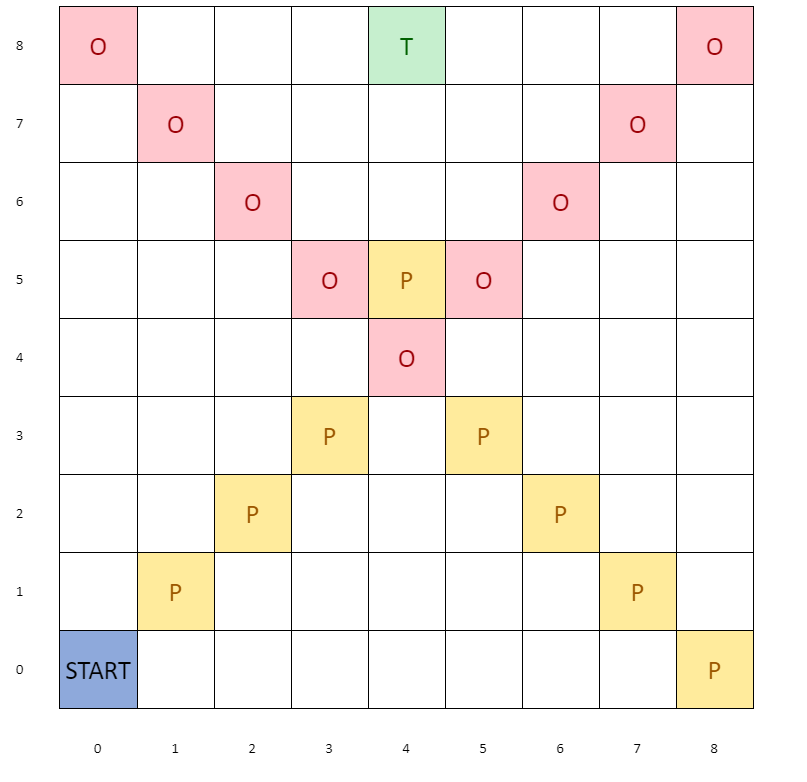
\includegraphics[width=\textwidth]{images/test5.png}
         \caption{Test 5}
         \label{fig:test15}
     \end{subfigure}
     \hfill
     \begin{subfigure}[b]{0.45\textwidth}
         \centering
         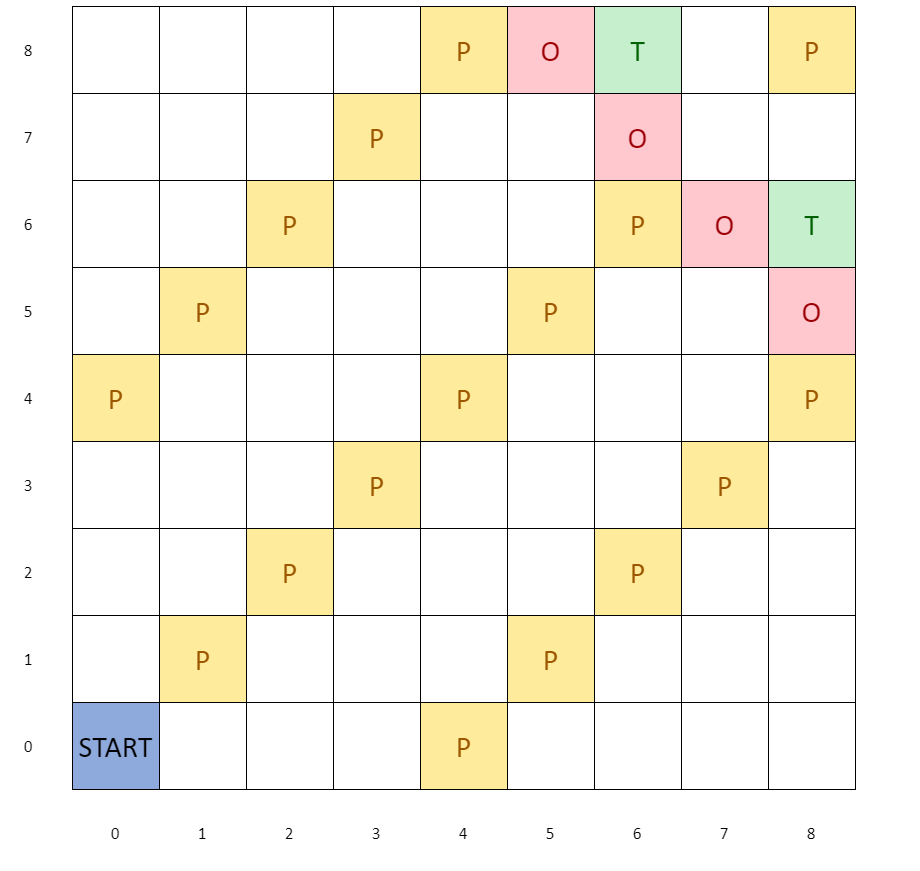
\includegraphics[width=\textwidth]{images/test6.png}
         \caption{Test 6}
         \label{fig:test16}
     \end{subfigure}
\end{figure}

\begin{figure}[H]
   	 \centering
     \begin{subfigure}[b]{0.45\textwidth}
         \centering
         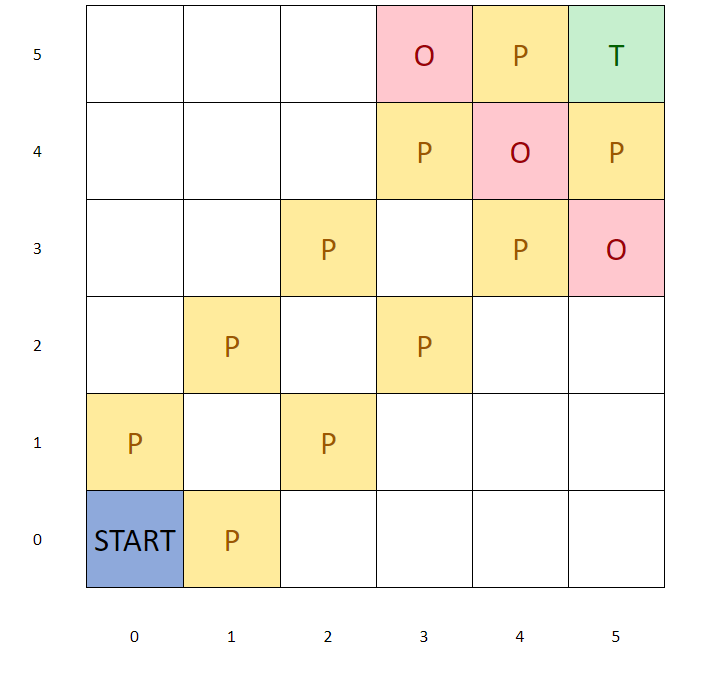
\includegraphics[width=\textwidth]{images/test7.png}
         \caption{Test 7}
         \label{fig:test17}
     \end{subfigure}
     \hfill
     \begin{subfigure}[b]{0.45\textwidth}
         \centering
         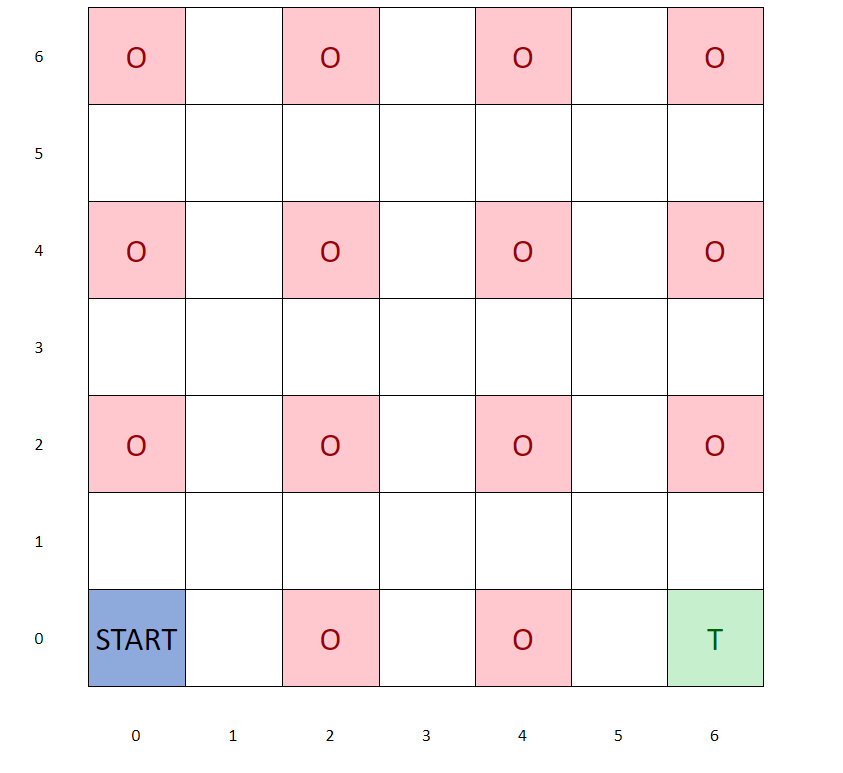
\includegraphics[width=\textwidth]{images/test8.png}
         \caption{Test 8}
         \label{fig:test18}
     \end{subfigure}
\end{figure}

\begin{figure}[H]
   	 \centering
     \begin{subfigure}[b]{0.45\textwidth}
         \centering
         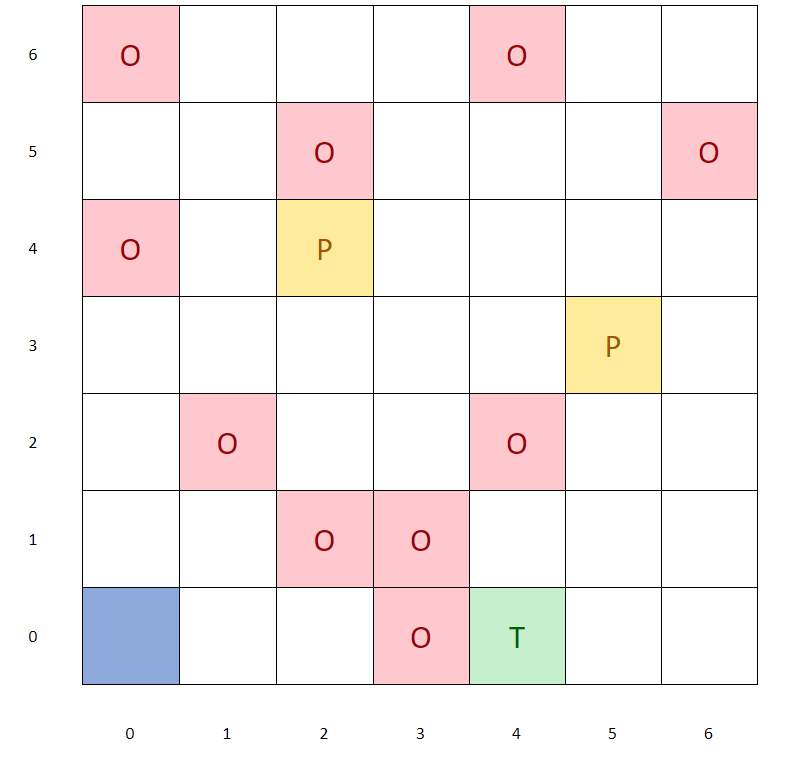
\includegraphics[width=\textwidth]{images/test9.png}
         \caption{Test 9}
         \label{fig:test19}
     \end{subfigure}
     \hfill
     \begin{subfigure}[b]{0.45\textwidth}
         \centering
         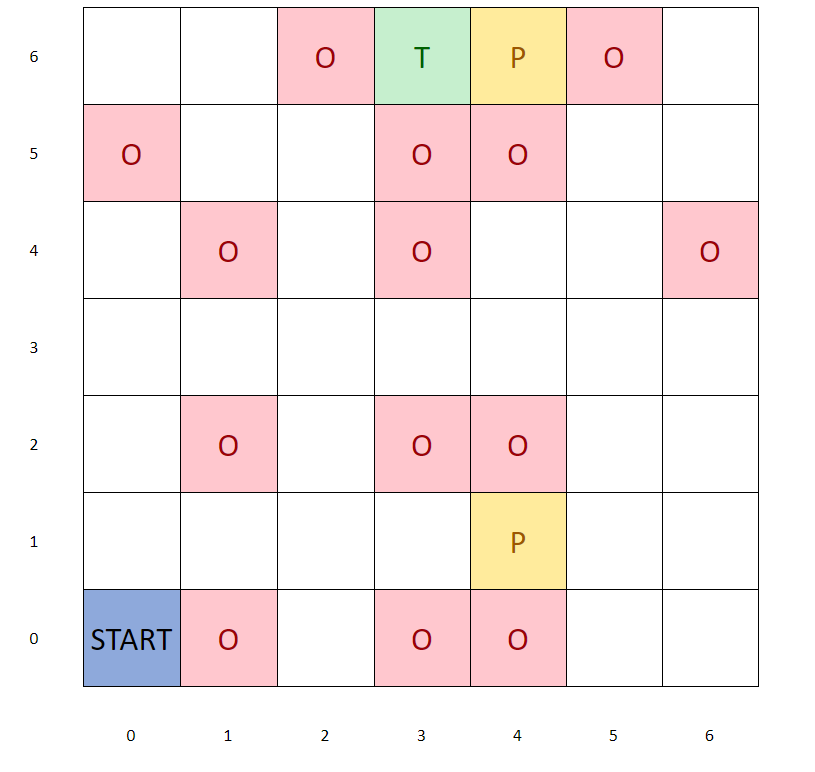
\includegraphics[width=\textwidth]{images/test10.png}
         \caption{Test 10}
         \label{fig:test110}
     \end{subfigure}
\end{figure}

\begin{figure}[H]
   	 \centering
     \begin{subfigure}[b]{0.45\textwidth}
         \centering
         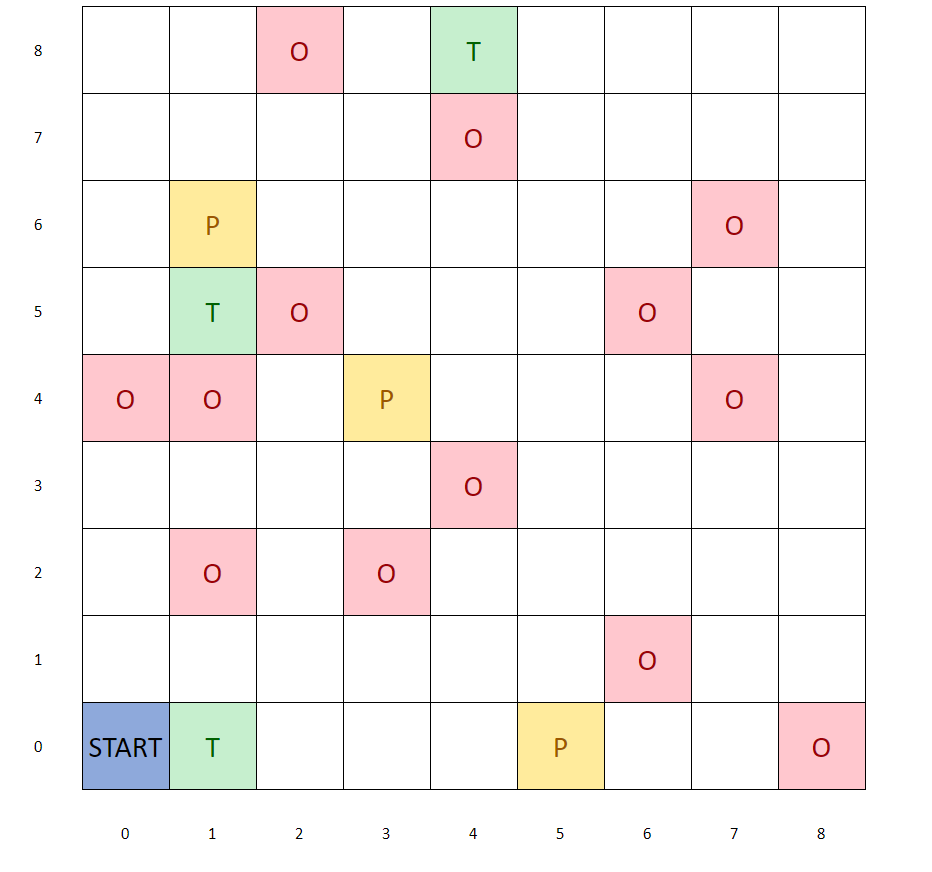
\includegraphics[width=\textwidth]{images/test11.png}
         \caption{Test 11}
         \label{fig:test111}
     \end{subfigure}
     \hfill
     \begin{subfigure}[b]{0.45\textwidth}
         \centering
         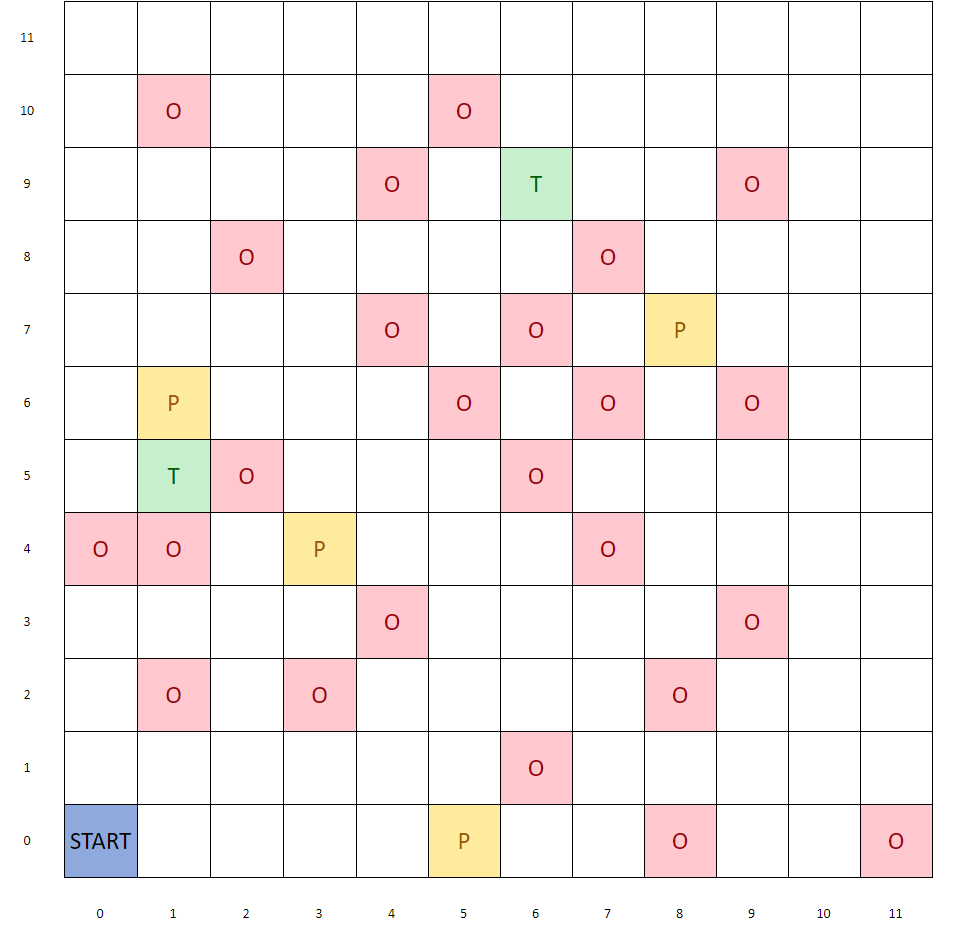
\includegraphics[width=\textwidth]{images/test12.png}
         \caption{Test 12}
         \label{fig:test112}
     \end{subfigure}
\end{figure}

\begin{figure}[H]
   	 \centering
     \begin{subfigure}[b]{0.45\textwidth}
         \centering
         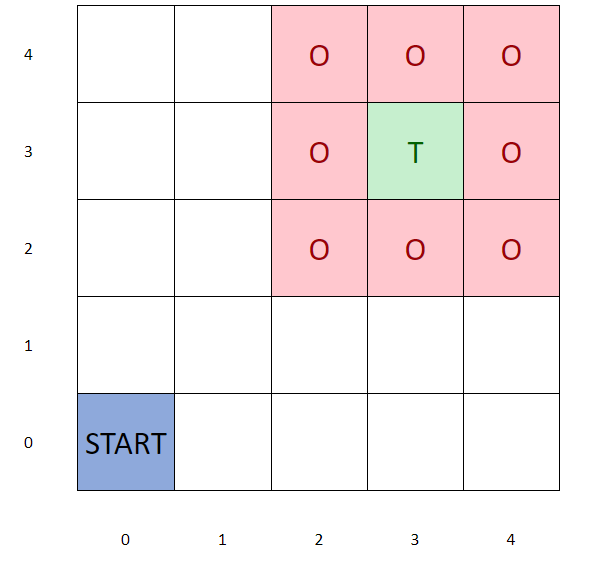
\includegraphics[width=\textwidth]{images/test13.png}
         \caption{Test 13}
         \label{fig:test113}
     \end{subfigure}
     \hfill
     \begin{subfigure}[b]{0.45\textwidth}
         \centering
         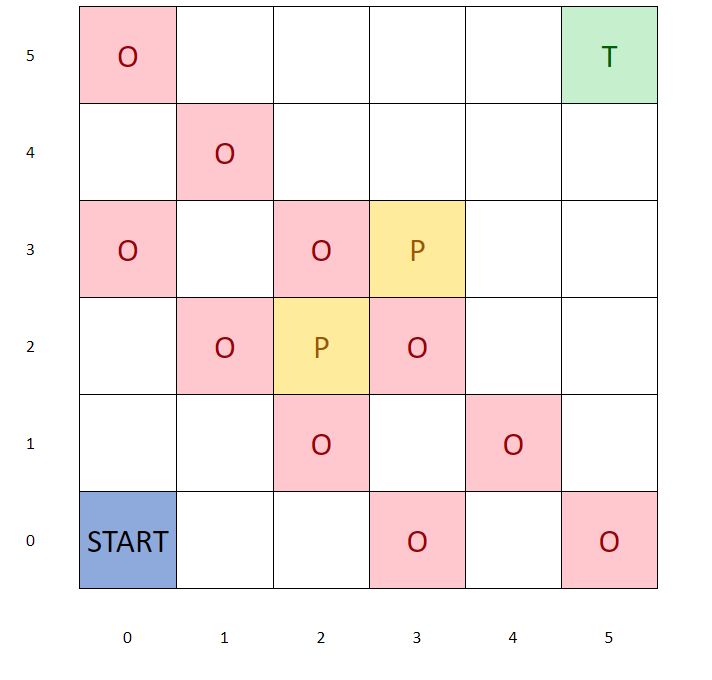
\includegraphics[width=\textwidth]{images/test14.png}
         \caption{Test 14}
         \label{fig:test114}
     \end{subfigure}
\end{figure}


\end{appendices}
\end{document}

